\documentclass{article}
\usepackage[utf8]{inputenc}
\usepackage{graphicx}
% \usepackage{captionsetup}
\begin{document}
\title{PCT Lab Report 1}
\author{Alexander Hiller (11850637)}
\maketitle

\newpage

\tableofcontents

\listoffigures

\newpage

\section{Method}

\section{Results}

  \subsection{RC Circuit}
    \begin{table}[h]
      \centering
      \caption{Tabulated experimentally measured and calculated results. Note that $\phi_r$ denotes the phase angle of $V_r$ and $\phi_c$ denotes the phase anlge of $V_c$. \\}
      {\renewcommand{\arraystretch}{1.2}
      \begin{tabular}{|c|c|c|c|c|c|c|c|}
        \toprule
        \hline
        $V_r$ &  ${V_c}$ &  $I_p$ & $R$ &  $\phi_r$ (radians) &  $\phi_r$ (degrees) & $\phi_c$ (radians) &  $\phi_c$ (degrees) \\
        \hline
        \midrule
        \hline 0 &    120.9 &    0.764 &    0.000 &               1.571 &              90.000 &               0.000 &               0.000  \\
        \hline 10 &    120.1 &    0.748 &   13.369 &               0.917 &              52.548 &              -0.654 &             -37.452 \\
        \hline 20 &    119.1 &    0.732 &   27.322 &               0.568 &              32.570 &              -1.002 &             -57.430 \\
        \hline 30 &    116.6 &    0.716 &   41.899 &               0.395 &              22.614 &              -1.176 &             -67.386 \\
        \hline 40 &    114.4 &    0.698 &   57.307 &               0.296 &              16.939 &              -1.275 &             -73.061 \\
        \hline 50 &    110.5 &    0.684 &   73.099 &               0.234 &              13.429 &              -1.336 &             -76.571 \\
        \hline 60 &    107.7 &    0.664 &   90.361 &               0.191 &              10.932 &              -1.380 &             -79.068 \\
        \hline 70 &    102.3 &    0.628 &  111.465 &               0.155 &               8.899 &              -1.415 &             -81.101 \\
        \hline 80 &     95.1 &    0.580 &  137.931 &               0.126 &               7.212 &              -1.445 &             -82.788 \\
        \hline 90 &     86.8 &    0.534 &  168.539 &               0.103 &               5.912 &              -1.468 &             -84.088 \\
        \hline 100 &     73.8 &    0.458 &  218.341 &               0.080 &               4.570 &              -1.491 &            -85.430 \\
        \hline 110 &     59.5 &    0.360 &  305.556 &               0.057 &               3.269 &              -1.514 &            -86.731 \\
        \hline
        \bottomrule
        \end{tabular}
        }
    \end{table}

  \subsection{Loci of RC Circuit}

    \begin{figure}[!h]
        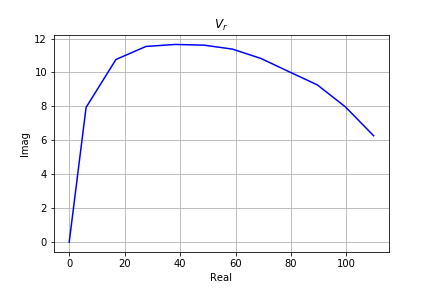
\includegraphics[width=0.8\textwidth]{RC_V_r_locus}
        \centering
        \caption{The locus of $V_r$}
    \end{figure}
    \begin{figure}[!h]
        \includegraphics[width=0.8\textwidth]{RC_V_C_locus}
        \centering
        \caption{The locus of $V_c$}
    \end{figure}
    \begin{figure}[!h]
        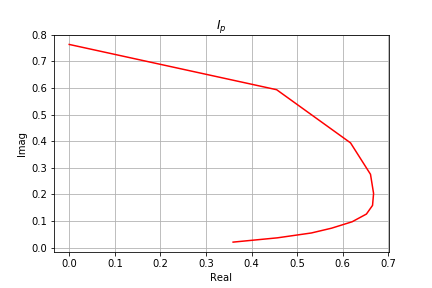
\includegraphics[width=0.8\textwidth]{RC_I_p_locus}
        \centering
        \caption{The locus of $I_p$}
    \end{figure}

  \subsection{RL Circuit}

  \subsection{RLC Circuit}

\section{Discussion}

\section{Conclusion}

\end{document}
